\chapter{Úvod}

\section{Motivace projektu, záměr práce}
%% motivace projektu (popsat přechod od samotné gramatiky jazyka k dalším pravidlům, která musí výsledný zdrojový kód splňovat)

% popis členění práce - co nalezne čtenář v jednotlivých kapitolách, jak je celé dílo strukturováno

Vymezení práce je graficky znázorněno na obrázku \ref{work_scope}.

TODO: sort and rewrite following paragraphs:

Množina pravidel vymezuje \uv{coding conventions} $\rightarrow$ zpřesnění modelu (omezení množiny instancí daného jazyka) daného gramatikou jazyka.

Analogie:
XML $\rightarrow$ well-formedness vs. validity (validace v tomto kontextu je analogická validaci xml dokumentu)

\begin{figure}[h!]
  \centering
  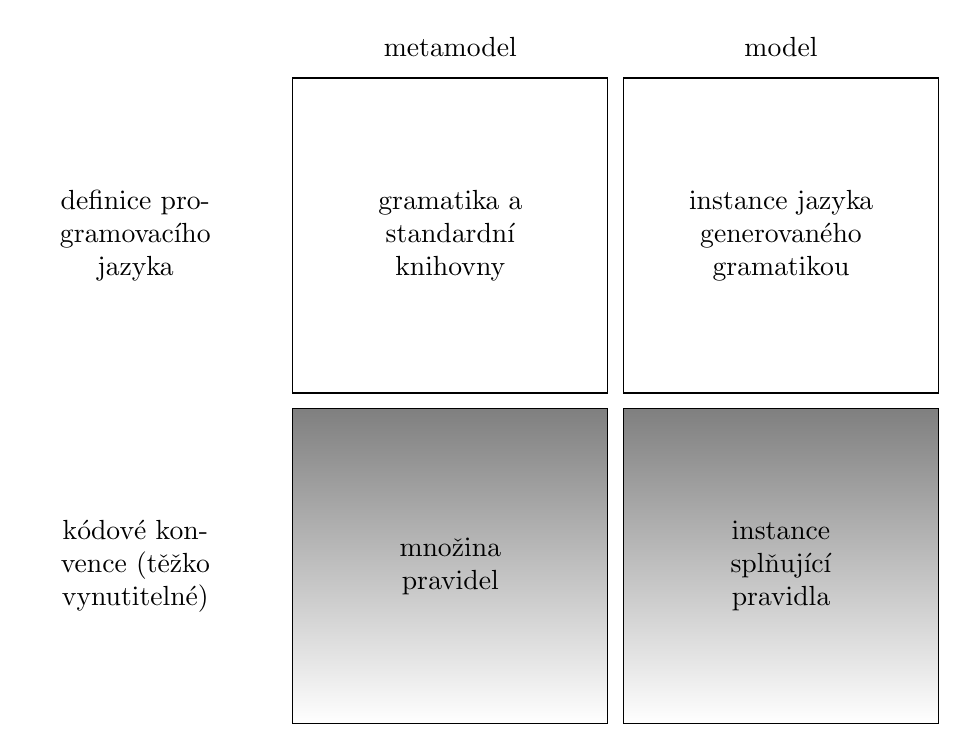
\begin{tikzpicture}
    \shadedraw  (0,0) rectangle (4,4);
    \shadedraw  (4.2,0) rectangle (8.2,4);
    \draw  (0,4.2) rectangle (4.0,8.2);
    \draw  (4.2,4.2) rectangle (8.2,8.2);

    \draw  (2,2) node[text width=2.5cm, text centered] {množina pravidel};
    \draw  (6.2,2) node[text width=2.5cm, text centered] {instance splňující pravidla};
    \draw  (2,6.2) node[text width=2.5cm, text centered] {gramatika a standardní knihovny};
    \draw  (6.2,6.2) node[text width=2.5cm, text centered] {instance jazyka generovaného gramatikou};

    \draw (-2,2) node[text width=2.5cm, text centered] {kódové konvence (těžko vynutitelné)};
    \draw (-2,6.2) node[text width=2.5cm, text centered] {definice programovacího jazyka};

    \draw (2,8.6) node[text width=2.5cm, text centered] {metamodel};
    \draw (6.2,8.6) node[text width=2.5cm, text centered] {model};
  \end{tikzpicture}
  \caption{Grafické znázornění zařazení práce.\label{work_scope}}
\end{figure}

% TODO: integrate following piece of text into main text flow
Množina pravidel může být zadávána neformálně (např.: \uv{třída nesmí záviset na více než čtyřech dalších nesystémových třídách}) nebo pomocí vhodně definovaného formalismu.

\section{Úvod do řešené problematiky}
% lehce rozebrat, čeho se bude práce týkat (spíše hodně highlevel, nezabředávat do detailů)

\subsection{Validace správného návrhu kódu}
\begin{itemize}
\item o co se jedná?
\item proč provádět validaci?
\end{itemize}

\subsection{Příklady pravidel}

\begin{itemize}
\item \uv{v běžném kódu by se něměla vyskytovat pole s modifikátorem \emph{public}, pouze \emph{private}, k~nimž se přistupuje pomocí \emph{getterů} a \emph{setterů}}
\item \uv{třídy z balíčku A nesmí záviset na jiných nesystémových \emph{třídách}, ale nejvýše na \emph{rozhraních} balíčku B} (programování proti rozhraní namísto proti konkrétní implementaci)
\item \uv{třídy v tomto balíčku smí mít maximálně pět metod, z nichž každá smí mít nejvýše tři parametry} (může být konvence v nějaké firmě)
\item law of Demeter
\end{itemize}
